\chapter{Experimentos Numéricos}

\section{Implementação Computacional da Tomografia por Impedância Elétrica}

\subsection{Discretização do problema}

Na descrição do modelo realizada na Seção \ref{sec:modelo-completo-eletrodos}, consideramos o corpo um domínio $\Omega \subset \R^2$. Inicialmente, ao longo de $\Omega$ é feita uma denominada triangulação, isto é, uma subdivisão do domínio em um conjunto de triângulos cujas arestas não contém vértices de outros triângulos em seu interior. Gera-se uma malha composta por $N$ triângulos $T_1,\dots,T_N$, definidos por $K$ vértices $P_1,\dots,P_K$. A Figura~\ref{fig:malha} ilustra uma triangulação feita em um disco unitário, que consiste do conjunto $D = \{(x,y) \in \R^2 | x^2+y^2 \leq 1\}$.

\begin{figure}[htbp]
    \centering
    \caption{Exemplo de triangulação de um disco unitário D.}
    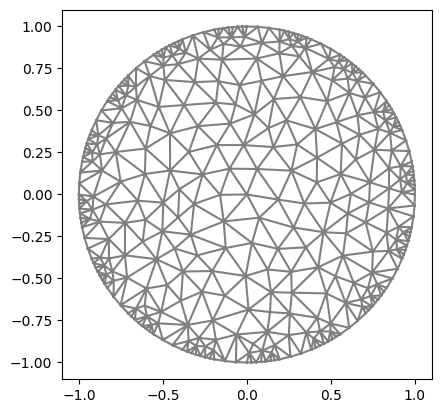
\includegraphics[scale=0.75]{figuras/malha.png}
    \label{fig:malha}
\end{figure}

No método de discretização utilizado, baseado no chamado Método de Elementos Finitos, as funções serão aproximadas por certos espaços de funções com dimensão finita, gerados por tipos de funções especiais. Desse modo, as funções a princípio definidas em um domínio com infinitos pontos, podem ser representadas como um vetor de coeficientes de uma combinação linear. Em particular, para a TIE são utilizados dois espaços: o gerado por funções características, e o gerado por funções afim por partes.

Para o primeiro tipo, consideramos as funções características $\chi_{T_j}$ de cada triângulo $T_j$, as quais indicam se os pontos estão no triângulo $T_j$ correspondente, tendo valor $1$ caso afirmativo e valor $0$ caso contrário. Estas são definidas em $\Omega$ e dadas por:

\begin{equation}
    \chi_{T_j} (x) = \begin{cases}
        1, x \in T_j , \\
        0, x \notin T_j.
    \end{cases}
\end{equation}

No problema específico da TIE, trataremos as condutividades $\gamma$ como funções do espaço gerado por funções características dos triângulos que compõem a triangulação. Isto é, dadas as funções características $\chi_{T_1}, \dots, \chi_{T_N}$ de cada triângulo da malha construída, consideramos que a condutividade é uma função $\gamma \in V_1 = span\{\chi_{T_1}, \dots,\chi_{T_N}\}$ no espaço gerado pelas funções características, podendo assim ser representada na forma:

\begin{equation} \label{eq:gamma-expansao}
    \gamma = \gamma_1 \chi_{T_1} + \dots + \gamma_N \chi_{T_N},
\end{equation}
onde $\gamma_1, \dots, \gamma_N \in \R$ são coeficientes específicos para cada função $\gamma$.

O segundo espaço consiste em funções contínuas afins em cada triângulo. Uma base para esse espaço é composto das funções $v_i$ tais que para cada vértice $P_i$
\begin{equation}
    v_i (P_j) = \begin{cases}
        1, i=j , \\
        0, i \neq j
    \end{cases}
\end{equation}
e são afins dentro de cada triângulo. Essencialmente, é definida uma função para cada vértice, atingindo valor 1 no vértice correspondente e assumindo valores intermediários linearmente em torno dele. No contexto da TIE, esse espaço de funções será utilizado para aproximação das funções de distribuição do potencial. De mesma forma, consideramos a função $u \in V_2 = span\{v_1, \dots, v_n\}$ no espaço gerado $V_2$ por essas funções indicadoras, de forma que:
\begin{equation}\label{eq:u-expansao}
    u = u_1 v_1 + \cdots + u_K v_K
\end{equation}
sendo $u_1,\dots, u_K\in \R$ coeficientes próprios de cada função $u$.

Com as aproximações de $u$ e $\gamma$ através desses espaços finitos, podemos representá-las por um vetor formado pelas coordenadas respectivas. Isto é, dada $\gamma$ com coordenadas $\gamma_1, \dots, \gamma_N$ como na Equação \eqref{eq:gamma-expansao}, podemos tratar $\gamma$ como um vetor $\overline \gamma \in \R^N$ dado por
\begin{equation}
    \overline \gamma = \left( \gamma_1, \dots, \gamma_N \right).
\end{equation}
Similarmente, trataremos $u$ como um vetor $u \in \R^K$ formado por suas coordenadas no espaço de funções $v_i$, como na Equação \eqref{eq:u-expansao}.


\subsection{Cálculo do Operador Direto}


A seguir, descrevemos como pode ser realizado o cálculo do Operador Direto descrito na Seção \ref{sec:modelo-completo-eletrodos} a partir das técnicas de discretização utilizadas. Conforme descrito na seção citada, dados um domínio $\Omega$ contendo $L$ eletrodos, o operador $F$ associa cada condutividade $\gamma$ a um operador $\Lambda_\gamma$, o qual leva cada padrão de correntes $I \in \R^L$ a um padrão de potenciais medidos $U\in \R^L$ correspondentes. Vimos que este é definido a partir da Equação \eqref{eq:cem-variacional}, dada por:
\begin{equation*}
    \iint_\Omega \gamma (x) \nabla u(x) \cdot \nabla v(x)\diff x + \sum_{l=1}^L \frac{1}{z_l}\int_{e_l} (u-U_l)(v - V_l)\diff s = \sum_{l=1}^L I_l V_l,
\end{equation*}
onde para cada $\gamma$ e cada padrão de correntes $I$ existe um único par $(u,U)$ que soluciona a equação dado qualquer par $(v,V)$ sob as condições definidas. 

Conforme detalhado por \citeonline{santana}, dada $\gamma$ no espaço $V_1$ e $u$ no espaço $V_2$ tendo respectivamente vetores de coordenadas $\overline \gamma\in \R^N$ e $\overline u \in \R^K$, como apresentado na subseção anterior, obter a solução $(u,U)$ para a Equação \eqref{eq:cem-variacional} equivale a solucionar um sistema linear
\begin{equation}\label{eq:variacional-linear}
    A \hat u = \overline{I},
\end{equation}
onde $\hat u \in \R^{K+L}$ é um vetor formado pelo ``empilhamento" do vetor de coordenadas $\overline u$ e do padrão de potenciais $U$, na forma:
\begin{equation}
    \hat u = \begin{pmatrix}
        \overline u \\
        U
    \end{pmatrix} = \begin{pmatrix}
        u_1 \\
        \vdots \\
        u_K \\
        U_1 \\
        \vdots \\
        U_L
    \end{pmatrix}.
\end{equation}
A matriz $A$ e o vetor $\overline I$ são formados a partir de cada lado da Equação~\eqref{eq:cem-variacional}, usando as impedâncias de contato, comprimento dos eletrodos, o vetor de correntes $I$ e o vetor $\overline \gamma$ \cite{santana}. Desse modo, a partir da versão discretizada de $\gamma$, podemos obter o padrão de correntes $U = F(\gamma)I = \Lambda_\gamma I$ a partir da solução $\hat u$ do sistema linear \eqref{eq:variacional-linear}.

Com isso, fixando um certo conjunto de padrões de correntes $\mathfrak I = (I^{(1)}\dots, I^{(l)})$, o operador $F_{\mathfrak I}$ conforme definido na Seção~\ref{sec:modelo-completo-eletrodos} pode ser calculado simplesmente a partir da relação:

\begin{equation}
    F_{\mathfrak I}(\gamma) = \begin{pmatrix}
        F(\gamma) I^{(1)} \\
        \vdots \\
        F(\gamma) I^{(l)}
    \end{pmatrix} = \begin{pmatrix}
        U^{(1)} \\
        \vdots \\
        U^{(l)}
    \end{pmatrix},
\end{equation}
onde o cálculo de cada $F(\gamma)I^{(j)}$ para todo $j \in \{1, \dots, l\}$ é realizado através do método descrito acima.


\subsection{Cálculo da Derivada do Operador Direto}


Como descrito na Seção \ref{sec:modelo-completo-eletrodos}, o operador $F$ do Modelo Completo de Eletrodos é diferenciável, o que faz também o Operador Direto $F_{\mathfrak I}$ diferenciável. Isso se torna de grande interesse para alguns dos métodos discutidos no Capítulo \ref{cap}, em especial os de Newton-Inexato. Com isso, podemos tentar obter métodos de trabalhar computacionalmente com a derivada do operador, ou ao menos as derivadas direcionais dado um vetor qualquer. Descrevemos a seguir como é realizado o cálculo da derivada desse operador, a partir das funções discretizadas.

Inicialmente, fixamos um conjunto de $l$ padrões correntes $I^{(1)},\dots, I{(l)}\in \R^L$ linearmente independentes. A partir disso, definimos para cada corrente $I^{(j)}$, com $j \in\{1, \dots, l\}$, o operador $F_j$ dado por
\begin{equation*}
    F_j(\gamma) = F(\gamma) I^{(j)}.
\end{equation*}
Desse modo, a partir do vetor de padrões de correntes $\mathfrak I = (I^{(1)}, \dots, I^{(l)}) \in \R^{l \times L}$, temos que:
\begin{equation}
    F_{\mathfrak I} (\gamma)  = \begin{pmatrix}
        F(\gamma) I^{(1)} \\
        \vdots \\
        F(\gamma) I^{(l)}
    \end{pmatrix} = 
    \begin{pmatrix}
        F_1(\gamma) \\
        \vdots \\
        F_l(\gamma)
    \end{pmatrix}.
\end{equation}

Note que, sendo $F$ diferenciável, segue que $F_j$ é diferenciável para todo $j \in \{1, \dots, l\}$, consequentemente tornando o Operador Direto $F_{\mathfrak I}$ também diferenciável. 

\citeonline{santana} detalha que dada uma função $\eta: \Omega \to \R$ em um espaço apropriado, calcular $F_j'(\gamma)\eta$, a derivada de $F_j$ em $\gamma$ aplicada em uma na direção $\eta$, equivale a obter a solução de uma equação variacional similar à Equação~\eqref{eq:cem-variacional}. Com as funções devidamente discretizadas, análogo ao desenvolvido para cálculo do Operador Direto, essa equação variacional é transformada em um sistema linear na forma

\begin{equation}
    A \hat \omega  = b,
\end{equation}
onde a matriz $A$ é a mesma do sistema \eqref{eq:variacional-linear} e o vetor $b$ é obtido a partir da versão discretizada de $\eta$. A solução $\hat \omega \in \R^{K +L}$ é dada na forma
\begin{equation} \label{eq:solucao-derivada-variacional}
    \hat \omega  = \begin{pmatrix}
        \omega_1 \\
        \vdots \\
        \omega_K \\
        \mathcal W_1 \\
        \vdots \\
        \mathcal W_L
    \end{pmatrix},
\end{equation}
onde o bloco $\mathcal{W}^{(j)} = (\mathcal W_1, \dots, \mathcal W_L)\in \R^L$ corresponde justamente a $F_j'(\gamma) \eta$. Isto é, 
\begin{equation}
    F_j'(\gamma) \eta = \mathcal{W}^{(j)}.
\end{equation}

Com isso, podemos calcular ainda $F_{\mathfrak I}'(\gamma) \eta$ visto que:
\begin{equation}
   F_{\mathfrak I}'(\gamma) \eta = \begin{pmatrix}
        F_1'(\gamma)\eta \\
        \vdots \\
        F_l'(\gamma)\eta
    \end{pmatrix} = \begin{pmatrix}
        \mathcal W^{(1)} \\
        \vdots \\
        \mathcal W^{(1)}
    \end{pmatrix}.
\end{equation}

Portanto, dada uma função $\eta$ com a mesma discretização utilizada para $\gamma$ descrita no início da seção, podemos calcular a derivada de $F_{\mathfrak I}$ em uma certa direção $\eta$ resolvendo sistemas lineares, obtidos a partir de determinadas equações variacionais.

Utilizando esse método, \citeonline{santana} mostra que ainda é possível calcular a Jacobiana de $F_{\mathfrak I}(\gamma)$ para uma $\gamma$ qualquer, a qual é dada por

\begin{equation}
    F_{\mathfrak I}'(\gamma) = \begin{pmatrix}
        F_1'(\gamma) \chi_{T_1} & \cdots & F_1'(\gamma) \chi_{T_1} \\
        \vdots & \ddots & \vdots \\
        F_l'(\gamma) \chi_{T_1} & \cdots & F_l'(\gamma) \chi_{T_N}
    \end{pmatrix},
\end{equation}
sendo $\chi_{T_j}$ a função característica em cada triângulo $T_j$, mostrando ainda um método otimizado para cálculo de cada componente nessa matriz, necessitando de menos soluções de sistemas lineares.

\vspace{1em}

Nesta seção, descrevemos de que forma o Modelo Completo de Eletrodos da TIE pode ser tratado computacionalmente e implementado por meio de métodos numéricos. Conforme comentado anteriormente, este trabalho não possui o intuito de explorar os aspectos teóricos da implementação computacional, sendo, portanto, tratada mais brevemente. Desse modo, recomenda-se para mais detalhes em torno da implementação computacional a consulta nos trabalhos já citados, em especial o de \citeonline{santana}. Por fim, para os experimentos executados no restante deste Capítulo, será utilizada uma biblioteca desenvolvida em Python por \citeonline{hafemann} que provém ferramentas para realizar as operações e cálculos descritos acima, cujos detalhes em torno da implementação podem ser vistos em sua documentação \footnote{Disponível em: \url{https://hafemanne.github.io/FEIT\_CBM34/}}.


\section{Experimentos com Dados Sintéticos}

Na seguinte seção, realizamos diferentes experimentos utilizando dados sintéticos, gerados por funções artificiais pré-definidas. Em situações práticas, não se conhece precisamente a função da condutividade elétrica $\gamma: \Omega \to \R$ que se quer reconstruir. Logo, pode-se ter apenas uma estimativa do erro cometido por uma aproximação $\gamma_n$ gerada pelos métodos de regularização, não se tendo o erro exato. 

Entretanto, nosso intuito nessa seção é justamente definir algumas funções de condutividade, gerar os dados de potenciais através delas para, a seguir, resolver o Problema Inverso e ter uma medição mais precisa do erro obtido em cada método. Com isso, conseguimos, ao menos na situação controlada, medir o quão precisas são as aproximações obtidas pelos métodos.

Começamos inicialmente gerando os dados de potenciais, a partir de algumas funções que serão definidas como solução conhecida que se deseja reconstruir. Em seguida, comparamos as soluções obtidas por diferentes métodos através de alguns cenários diferentes. Primeiramente, vemos como cada método se comporta para diferentes níveis de ruído em uma mesma função. Em seguida, analisamos as reconstruções obtidas para cada solução pré-definida. 

Os métodos selecionados para comparação serão os métodos de Landweber (LW), Levenberg - Marquadt (LM), REGINN com iteração interna Gradiente (NG), e REGINN com iteração interna de Tikhonov (NT).

